\documentclass[11pt]{article}

% Text extraction: map ligatures to letters and use T1 encoding under pdfLaTeX.
\usepackage{iftex}
\ifPDFTeX
  \input{glyphtounicode}
  \pdfgentounicode=1
  \usepackage[T1]{fontenc}
  \usepackage{lmodern}
\fi
\usepackage[a4paper,margin=2.5cm]{geometry}
\usepackage{microtype}
\usepackage{amsmath,amssymb}
\usepackage{graphicx}
\usepackage{booktabs}
\usepackage{array}
\usepackage{xcolor}
\usepackage[numbers,sort&compress]{natbib}
\usepackage[hidelinks]{hyperref}
\usepackage{caption}
\captionsetup{font=small,labelfont=bf}

\newcommand{\meanpm}[2]{#1\,$\pm$\,#2}
\newcommand{\protocol}[1]{\textsf{#1}}
\providecommand{\pending}{\textit{[pending]}}
\newcommand{\AblBgEst}{\pending}
\newcommand{\AblBgHi}{\pending}
\newcommand{\AblBgLo}{\pending}
\newcommand{\AblBgP}{\pending}
\newcommand{\AblFlatEst}{\pending}
\newcommand{\AblFlatHi}{\pending}
\newcommand{\AblFlatLo}{\pending}
\newcommand{\AblFlatP}{\pending}
\newcommand{\AblGreyEst}{\pending}
\newcommand{\AblGreyHi}{\pending}
\newcommand{\AblGreyLo}{\pending}
\newcommand{\AblGreyP}{\pending}
\newcommand{\AblLowEst}{\pending}
\newcommand{\AblLowHi}{\pending}
\newcommand{\AblLowLo}{\pending}
\newcommand{\AblLowP}{\pending}
\newcommand{\CamLeakEst}{\pending}
\newcommand{\CamLeakHi}{\pending}
\newcommand{\CamLeakLo}{\pending}
\newcommand{\CamLeakP}{\pending}
\newcommand{\CricBaccDf}{18.0}
\newcommand{\CricBaccEst}{19.64}
\newcommand{\CricBaccHi}{21.13}
\newcommand{\CricBaccKRp}{$<$0.001}
\newcommand{\CricBaccLo}{18.15}
\newcommand{\CricBaccP}{$<$0.001}
\newcommand{\CricBaccSupported}{supported}
\newcommand{\CricErrorRatio}{2.27}
\newcommand{\CricFoneDf}{6.3}
\newcommand{\CricFoneEst}{20.59}
\newcommand{\CricFoneHi}{22.05}
\newcommand{\CricFoneKRp}{$<$0.001}
\newcommand{\CricFoneLo}{19.13}
\newcommand{\CricFoneP}{$<$0.001}
\newcommand{\CricFoneSupported}{supported}
\newcommand{\CricPOneAcc}{90.48}
\newcommand{\CricPOneBacc}{78.53}
\newcommand{\CricPTwoAcc}{78.40}
\newcommand{\CricPTwoBacc}{58.89}
\newcommand{\CricPrimeDf}{17.5}
\newcommand{\CricPrimeEst}{12.11}
\newcommand{\CricPrimeHi}{13.03}
\newcommand{\CricPrimeKRp}{$<$0.001}
\newcommand{\CricPrimeLo}{11.19}
\newcommand{\CricPrimeP}{$<$0.001}
\newcommand{\CricPrimeSupported}{supported}
\newcommand{\DecompDiv}{0.00}
\newcommand{\DecompGap}{0.97}
\newcommand{\DecompLeak}{1.59}
\newcommand{\DivEst}{0.00}
\newcommand{\DivHi}{0.64}
\newcommand{\DivLo}{\textminus{}0.65}
\newcommand{\DivP}{0.99}
\newcommand{\DonorShiftEst}{3.09}
\newcommand{\DonorShiftHi}{5.15}
\newcommand{\DonorShiftLo}{1.04}
\newcommand{\DonorShiftP}{0.02}
\newcommand{\FeightEst}{\pending}
\newcommand{\FeightHi}{\pending}
\newcommand{\FeightLo}{\pending}
\newcommand{\FeightP}{\pending}
\newcommand{\FeightPholm}{\pending}
\newcommand{\FeightStatus}{\pending}
\newcommand{\FeightSupported}{\pending}
\newcommand{\FfiveEst}{\pending}
\newcommand{\FfiveHi}{\pending}
\newcommand{\FfiveLo}{\pending}
\newcommand{\FfiveP}{\pending}
\newcommand{\FfivePholm}{\pending}
\newcommand{\FfiveStatus}{\pending}
\newcommand{\FfiveSupported}{\pending}
\newcommand{\FfourEst}{\pending}
\newcommand{\FfourHi}{\pending}
\newcommand{\FfourLo}{\pending}
\newcommand{\FfourP}{\pending}
\newcommand{\FfourPholm}{\pending}
\newcommand{\FfourStatus}{\pending}
\newcommand{\FfourSupported}{\pending}
\newcommand{\FollowupCommit}{80171fe}
\newcommand{\FollowupTime}{2026-10-19 14:02 IST}
\newcommand{\FoneCells}{1,144}
\newcommand{\FoneConcordant}{10.02}
\newcommand{\FoneContrast}{\textminus{}0.52}
\newcommand{\FoneContrastHi}{4.66}
\newcommand{\FoneContrastLo}{\textminus{}5.75}
\newcommand{\FoneDiscordant}{10.55}
\newcommand{\FoneEst}{\textminus{}4.29}
\newcommand{\FoneHi}{\textminus{}1.37}
\newcommand{\FoneLo}{\textminus{}8.60}
\newcommand{\FoneP}{$<$0.001}
\newcommand{\FonePholm}{\pending}
\newcommand{\FoneSlides}{230}
\newcommand{\FoneSupported}{\pending}
\newcommand{\FsevenEst}{\pending}
\newcommand{\FsevenHi}{\pending}
\newcommand{\FsevenLo}{\pending}
\newcommand{\FsevenP}{\pending}
\newcommand{\FsevenPholm}{\pending}
\newcommand{\FsevenStatus}{\pending}
\newcommand{\FsevenSupported}{\pending}
\newcommand{\FsixEst}{\pending}
\newcommand{\FsixHi}{\pending}
\newcommand{\FsixLo}{\pending}
\newcommand{\FsixP}{\pending}
\newcommand{\FsixPholm}{\pending}
\newcommand{\FsixStatus}{\pending}
\newcommand{\FsixSupported}{\pending}
\newcommand{\FthreeEst}{\pending}
\newcommand{\FthreeHi}{\pending}
\newcommand{\FthreeLo}{\pending}
\newcommand{\FthreeP}{\pending}
\newcommand{\FthreePholm}{\pending}
\newcommand{\FthreeStatus}{\pending}
\newcommand{\FthreeSupported}{\pending}
\newcommand{\FtwoEst}{\pending}
\newcommand{\FtwoHi}{\pending}
\newcommand{\FtwoLo}{\pending}
\newcommand{\FtwoP}{\pending}
\newcommand{\FtwoPholm}{\pending}
\newcommand{\FtwoStatus}{\pending}
\newcommand{\FtwoSupported}{\pending}
\newcommand{\GrlConvRstar}{55.1}
\newcommand{\GrlConvRzero}{29.5}
\newcommand{\GrlResGapMax}{0.70}
\newcommand{\GrlResGapMin}{0.28}
\newcommand{\GrlResGapZero}{1.17}
\newcommand{\GrlResRstar}{17.6}
\newcommand{\GrlResRzero}{24.7}
\newcommand{\HfiveEst}{0.06}
\newcommand{\HfiveHi}{0.12}
\newcommand{\HfiveLo}{\textminus{}0.01}
\newcommand{\HfiveP}{0.08}
\newcommand{\HfivePholm}{0.16}
\newcommand{\HfiveStatus}{tested}
\newcommand{\HfiveSupported}{not supported}
\newcommand{\HfourBgEst}{0.63}
\newcommand{\HfourBgHi}{1.33}
\newcommand{\HfourBgLo}{\textminus{}0.07}
\newcommand{\HfourBgP}{0.07}
\newcommand{\HfourEst}{0.42}
\newcommand{\HfourHi}{1.18}
\newcommand{\HfourLo}{\textminus{}0.35}
\newcommand{\HfourP}{0.23}
\newcommand{\HfourPholm}{0.23}
\newcommand{\HfourSupported}{not supported}
\newcommand{\HoneArchCIPositive}{11}
\newcommand{\HoneArchMax}{1.44}
\newcommand{\HoneArchMin}{0.66}
\newcommand{\HoneBaccDf}{38.8}
\newcommand{\HoneBaccEst}{0.98}
\newcommand{\HoneBaccHi}{1.40}
\newcommand{\HoneBaccKRp}{$<$0.001}
\newcommand{\HoneBaccLo}{0.60}
\newcommand{\HoneBaccP}{$<$0.001}
\newcommand{\HoneBaccSupported}{supported}
\newcommand{\HoneBootHi}{1.39}
\newcommand{\HoneBootLo}{0.59}
\newcommand{\HoneBootP}{$<$0.001}
\newcommand{\HoneDf}{38.8}
\newcommand{\HoneEst}{0.97}
\newcommand{\HoneFoneDf}{38.8}
\newcommand{\HoneFoneEst}{0.96}
\newcommand{\HoneFoneHi}{1.39}
\newcommand{\HoneFoneKRp}{$<$0.001}
\newcommand{\HoneFoneLo}{0.59}
\newcommand{\HoneFoneP}{$<$0.001}
\newcommand{\HoneFoneSupported}{supported}
\newcommand{\HoneGlmmLogOR}{0.304}
\newcommand{\HoneGlmmP}{$<$0.001}
\newcommand{\HoneHi}{1.39}
\newcommand{\HoneKRp}{$<$0.001}
\newcommand{\HoneLo}{0.59}
\newcommand{\HoneModel}{full}
\newcommand{\HoneP}{$<$0.001}
\newcommand{\HonePositiveArchs}{12}
\newcommand{\HoneSignFlipP}{$<$0.001}
\newcommand{\HoneSupported}{supported}
\newcommand{\HthreeEst}{1.73}
\newcommand{\HthreeHi}{2.51}
\newcommand{\HthreeLo}{0.95}
\newcommand{\HthreeP}{0.006}
\newcommand{\HthreePholm}{0.02}
\newcommand{\HthreeRepEst}{\pending}
\newcommand{\HthreeRepHi}{\pending}
\newcommand{\HthreeRepLo}{\pending}
\newcommand{\HthreeRepP}{\pending}
\newcommand{\HthreeSupported}{supported}
\newcommand{\HtwoDf}{8.8}
\newcommand{\HtwoEst}{12.08}
\newcommand{\HtwoHi}{12.99}
\newcommand{\HtwoKRp}{$<$0.001}
\newcommand{\HtwoLo}{11.16}
\newcommand{\HtwoP}{$<$0.001}
\newcommand{\HtwoPholm}{$<$0.001}
\newcommand{\HtwoSupported}{supported}
\newcommand{\InteractionEst}{\textminus{}0.20}
\newcommand{\InteractionHi}{0.55}
\newcommand{\InteractionLo}{\textminus{}0.94}
\newcommand{\InteractionP}{0.60}
\newcommand{\KendallHi}{0.86}
\newcommand{\KendallLo}{0.42}
\newcommand{\KendallTau}{0.82}
\newcommand{\LeakOriginalEst}{1.73}
\newcommand{\LeakOriginalHi}{2.10}
\newcommand{\LeakOriginalLo}{1.35}
\newcommand{\LeakOriginalP}{$<$0.001}
\newcommand{\MaskReductionEst}{\pending}
\newcommand{\MaskReductionHi}{\pending}
\newcommand{\MaskReductionLo}{\pending}
\newcommand{\MaskReductionP}{\pending}
\newcommand{\MoneCrops}{3,664}
\newcommand{\MoneEst}{1.29}
\newcommand{\MoneHi}{1.50}
\newcommand{\MoneLo}{1.10}
\newcommand{\MtwoOverlapLogOdds}{0.45}
\newcommand{\MtwoOverlapP}{$<$0.001}
\newcommand{\MtwoSiblingsLogOdds}{0.15}
\newcommand{\MtwoSiblingsP}{0.01}
\newcommand{\OrderingPassed}{4/12}
\newcommand{\PilotDf}{9.1}
\newcommand{\PilotEst}{1.37}
\newcommand{\PilotP}{0.005}
\newcommand{\PilotSE}{0.38}
\newcommand{\PowerChosen}{0.977}
\newcommand{\PowerInflated}{0.782}
\newcommand{\PtwoPthreeDf}{25.7}
\newcommand{\PtwoPthreeEst}{0.03}
\newcommand{\PtwoPthreeHi}{0.56}
\newcommand{\PtwoPthreeKRp}{0.90}
\newcommand{\PtwoPthreeLo}{\textminus{}0.49}
\newcommand{\PtwoPthreeP}{0.90}
\newcommand{\PtwoPthreeSupported}{not supported}
\newcommand{\RegistrationCommit}{a62e8e7}
\newcommand{\RegistrationTime}{2026-10-18 05:07 IST}
\newcommand{\ReorderedPairs}{6/66}
\newcommand{\RouteShare}{24}
\newcommand{\SipErrorRatio}{1.34}
\newcommand{\SipPOneAcc}{97.14}
\newcommand{\SipPTwoAcc}{96.18}
\newcommand{\TransplantCleanHarmony}{2.29}
\newcommand{\TransplantLeakOther}{1.70}
\newcommand{\TransplantLeakSibling}{1.72}
\newcommand{\TransplantLeakUnseen}{1.30}


\title{Do We Train on Test Cells?\\[2pt]
\large A Preregistered Audit of Hierarchical Leakage in Cervical Cytology Benchmarks}
\author{Snehasish Ghosh\textsuperscript{1}, Soham Mitra\textsuperscript{2}, Nibaran Das\textsuperscript{2}\\[4pt]
\small \textsuperscript{1}Indian Institute of Science, Bengaluru, India\quad
\textsuperscript{2}Jadavpur University, Kolkata, India}
\date{}

\begin{document}
\maketitle

\begin{abstract}
Public cervical cytology benchmarks release many cell crops cut from far fewer microscope
fields or slide images, and are usually split at the crop level, so test cells share their
acquisition with training cells. A first study showed that this structure is pervasive and that
the shared parent is recognisable, but six per-architecture tests could not show that it inflates
accuracy. In a second, preregistered study (1,341 models) we test the question once, with a
mixed model sized by simulation: across twelve architectures and twenty new seeds, crop-level
splitting raised SIPaKMeD accuracy by \HoneEst\ percentage points (95\% CI \HoneBootLo--\HoneBootHi),
so parent-level splitting reveals \SipErrorRatio\ times the error rate. On CRIC, whose slide
images hold many cells of several classes, the inflation was \HtwoEst\ points. A factorial
that holds crop and field counts fixed shows that the inflation is leakage (\HthreeEst\ points)
and not the extra training diversity crop-level splits bring (diversity effect \DivEst\ points). Eight further registered
experiments (1,580 runs) locate the leaked signal by elimination. It needs no background and,
in an exploratory split, does not depend on shared pixels; it is not a slide-level label prior; and it is not carried by
linearly decodable field identity: erasing or adversarially suppressing that identity cut probe
recoverability by up to \RecoveryCutMax\% without moving the gap. It is instead tied to how a
field renders its cells: matching a test cell's colour statistics to an unseen field removed
most of it, although colour augmentation during training did not prevent it. Grad-CAM maps of
leaking and non-leaking models were indistinguishable. Neither probes, saliency maps, nor
augmentation can certify an evaluation; parent-disjoint splits can. We release the provenance
maps, splits, run records, and a risk calculator that predicts a benchmark's exposure from its
crop-to-parent table.

\end{abstract}

\section{Introduction}

Public cervical cytology datasets are usually released as cell crops, and most of those
crops are cut from a much smaller number of microscope fields or slide images. When a
benchmark is split at the crop level, crops from one field can land on both sides of
the train--test boundary. File-level disjointness then looks like independence while the
test set shares stain, illumination, focus, background, and sometimes literal pixels
with the training set.

This paper separates three claims that are easy to conflate:
\emph{structural non-independence} (test observations share a parent with training
observations), \emph{shortcut availability} (the shared parent leaves a learnable
fingerprint), and \emph{consequence} (classifiers score higher because they use it).
Our first study (Study~1) established the first two for four public datasets: random
crop splitting placed a training parent behind 92.6\% of SIPaKMeD and 99.97\% of CRIC test
cells, more than half of SIPaKMeD test crops shared source pixels with a training crop,
and a 424-way parent probe reached 109 times chance (79 times with the cell inpainted
away), while the one-cell-per-image Herlev control stayed at exactly zero. It did not
establish the third. All six architectures scored higher under crop-level than
parent-level splitting, by 0.72--2.25 percentage points, yet none of the six
per-architecture tests survived Benjamini--Hochberg correction.

That design had four weaknesses, and this paper is a second, separately preregistered
study (Study~2) built to remove them:
\begin{enumerate}
\item \textbf{Specification.} One question was asked six times. We replace the six tests
  with a single mixed-effects test of the protocol effect, sized by simulation from the
  Study~1 pilot (twelve architectures, twenty new seeds; Section~\ref{sec:h1}).
\item \textbf{Availability versus use.} We test whether classifiers \emph{use} acquisition
  context with counterfactual background transplants (Section~\ref{sec:transplant}) and
  whether the inflation tracks the fingerprint when an adversary suppresses it
  (Section~\ref{sec:grl}).
\item \textbf{Leakage versus diversity.} At equal crop counts, crop-level training sets
  contain about 18\% more distinct parents than parent-level ones, so the protocol
  contrast also changes training diversity. A leakage-by-diversity factorial over one
  common test set separates the two (Section~\ref{sec:factorial}).
\item \textbf{One rescored benchmark.} We rescore CRIC, whose cells are drawn from 400
  multi-class slide images (Section~\ref{sec:cric}).
\end{enumerate}
Every Study~2 split, model, seed, endpoint, and test was committed before the first
Study~2 model was trained. All results are reported, including any that do not support
our hypotheses.

\section{Related work}

\paragraph{Leakage and duplicates.} Kapoor and Narayanan catalogue leakage as a cause of
irreproducible machine-learning science across fields~\citep{kapoor2023leakage}. Barz and
Denzler showed that near-duplicates of CIFAR test images inflate reported accuracy and
released a purged test set~\citep{barz2020cifair}; Laroca et al.\ found the same for
license plates~\citep{laroca2023lpr}. In medical imaging, patient identity is recoverable
from chest radiographs~\citep{packhauser2022reidentification}, so image-level splits of
multi-image patients can share identity across the boundary. Our setting is a hierarchy
rather than duplication: sibling crops are different cells from one acquisition unit.

\paragraph{Shortcut learning.} Networks often solve a task through cues that are
predictive in the training distribution but unrelated to the intended concept
\citep{geirhos2020shortcut}. Medical examples include hospital and scanner signatures in
pneumonia detection~\citep{zech2018pneumonia}, dataset-source artifacts in COVID-19
radiograph models~\citep{degrave2021covid}, and models that predict dietary habits from
knee radiographs~\citep{hill2024shortcutting}; see also the methodological review of
Varoquaux and Cheplygina~\citep{varoquaux2022failures}. Xiao et al.\ measured background
reliance by recombining ImageNet foregrounds with backgrounds from other
classes~\citep{xiao2021noise}; our transplant arm adapts that design to acquisition
context in cytology.

\paragraph{Removing nuisance information.} Gradient reversal trains a representation
that is uninformative about a nuisance variable by adversarially training a nuisance
predictor~\citep{ganin2015backprop,ganin2016dann}. We use it as an intervention on the
parent fingerprint rather than for domain adaptation.

\paragraph{Variance and inference in benchmarks.} Benchmark comparisons inherit
variance from data splits and initialization~\citep{bouthillier2021variance}. Crossed
mixed-effects models with maximal random-effects structure~\citep{barr2013maximal,bates2015lme4}
and Satterthwaite or Kenward--Roger degrees of freedom~\citep{satterthwaite1946,kenward1997small,kuznetsova2017lmertest}
are the standard way to generalise a fixed effect over both items and conditions;
simulation-based power analysis handles their non-closed-form power~\citep{green2016simr}.

\section{Datasets and provenance}
\label{sec:data}

\begin{table}[t]
\centering\footnotesize
\setlength{\tabcolsep}{4pt}
\caption{Audited datasets and their independent units.}
\label{tab:datasets}
\begin{tabular}{lllrrrl}
\toprule
Dataset & Observation & Parent & Obs. & Parents & Obs./parent & Released task \\
\midrule
SIPaKMeD & cell crop & cluster field & 4,049 & 966 & 4.19 & 5-class classification \\
Cx22 & generated ROI & CCEDD source image & 1,320 & 514 & 2.57 & segmentation \\
CRIC & classified cell & slide image & 11,534 & 400 & 28.84 & 6-class classification \\
Herlev & single-cell image & the image itself & 917 & 917 & 1.00 & 7-class classification \\
\bottomrule
\end{tabular}
\end{table}


Table~\ref{tab:datasets} lists the four audited datasets and their independent units.
SIPaKMeD crops come from cluster fields~\citep{plissiti2018sipakmed}; Cx22 regions come
from CCEDD source images~\citep{liu2022cx22}; CRIC cells come from 400 conventional Pap
smear images~\citep{rezende2021cric}; Herlev releases one cell per image and serves as the
negative control~\citep{jantzen2005pap}. For SIPaKMeD, two independent recovery branches
(filename parsing, and template matching of each crop against every same-class field)
agree on all 4,049 crops, and every recovered box lies inside its field. Raw images are
never redistributed; the released artifacts are identifiers, coordinates, hashes, and
split assignments.

\section{Structural leakage and the parent fingerprint}
\label{sec:structure}

For a parent with $k$ crops allocated independently with test fraction $q$, the probability
that it straddles the split is $1-(1-q)^k-q^k$, a test crop has a training sibling with
probability $1-q^{k-1}$, and it has $(1-q)(k-1)$ training siblings on average. Averaging
these closed forms over the recovered parents predicts the structural leakage of a
random crop split before any split is drawn (Table~\ref{tab:structure}); the observed
values agree within Monte Carlo error. The same closed forms give the
\emph{training-diversity ratio} between crop-level and parent-level splits of equal size,
$\sum_j\{1-q^{k_j}\}/\{(1-q)m\}$ for $m$ parents, which is 1.18 for SIPaKMeD and 1.25 for
CRIC. The \texttt{cytofair risk-report} command computes all of these from any
crop-to-parent table.

\begin{table}[t]
\centering\footnotesize
\setlength{\tabcolsep}{4pt}
\caption{Structural leakage of a random 80:20 crop split. Straddle and test-crop leakage are percentages (observed: mean\,$\pm$\,SD over five seeds); siblings, diversity ratio, and class--parent dependence are closed-form expectations (\texttt{cytofair risk-report}); literal overlap is the percentage of test observations sharing source pixels with a training observation (same five seeds). P2 and P3 are exactly zero on every column.}
\label{tab:structure}
\begin{tabular}{lrrrrrrr}
\toprule
Dataset & Analytic & Observed & Test w/ train parent & Siblings & Diversity & Class dep. & Literal \\
\midrule
SIPaKMeD & 44.8 & 45.63\,$\pm$\,1.04 & 92.62\,$\pm$\,0.40 & 5.2 & 1.18 & 1.00 & 52.62\,$\pm$\,1.97 \\
Cx22 & 33.9 & 34.01\,$\pm$\,1.10 & 85.23\,$\pm$\,3.51 & 1.9 & 1.16 & -- & 34.02\,$\pm$\,1.80 \\
CRIC & 94.9 & 94.35\,$\pm$\,1.10 & 99.97\,$\pm$\,0.08 & 35.6 & 1.25 & 0.68 & 71.54\,$\pm$\,0.90 \\
Herlev & 0.0 & 0.00\,$\pm$\,0.00 & 0.00\,$\pm$\,0.00 & 0.0 & 1.00 & -- & 0.00 \\
\bottomrule
\end{tabular}
\end{table}


The fingerprint is learnable. A ResNet-18 trained to identify 424 SIPaKMeD fields from
two crops each recognised held-out sibling crops at 25.7\% accuracy (chance 0.24\%), still
reached 18.7\% from inpainted, cell-removed backgrounds, and fell to chance under shuffled
labels (Study~1). In SIPaKMeD every field belongs to one class, so recognising the field
implies the label. In CRIC, slide identity explains 1.23 of the 1.82 bits of class
entropy (68\%).

\section{Study 2 design}
\label{sec:design}

\subsection{Governance}

Study~2 was registered as an amendment to the original plan
(\texttt{PREREGISTRATION\_STUDY2.md}, commit \texttt{\RegistrationCommit},
\RegistrationTime). Before registration, every split, design table, transplant plan, and
input cache was generated and hashed, and one-epoch smoke tests were run only on
crop-level splits, so no protocol contrast could be observed. Study~1 runs serve only as
pilot estimates; Study~2 seeds are disjoint from Study~1 seeds. While validating the
analysis code we fitted the registered model to the Study~1 runs; that post hoc reanalysis
is reported in Appendix~\ref{app:pilot} and is not evidence for Study~2.

\subsection{Common training recipe}

Every run fine-tunes an ImageNet-initialised backbone with a new linear head: AdamW at
$10^{-4}$ with weight decay $10^{-4}$, batch 64, 20 epochs, final-epoch evaluation, no
validation split, early stopping, or checkpoint selection; random resized crops (scale
0.8--1.0) with horizontal and vertical flips. Twelve backbones span classic and modern
designs: ResNet-18 and -50~\citep{he2016resnet}, DenseNet-121~\citep{huang2017densenet},
MobileNet-V2~\citep{sandler2018mobilenetv2}, EfficientNet-B0~\citep{tan2019efficientnet},
ViT-B/16~\citep{dosovitskiy2021vit}, ConvNeXt-T~\citep{liu2022convnext},
Swin-T~\citep{liu2021swin}, RegNetY-1.6GF~\citep{radosavovic2020regnet},
EfficientNetV2-S~\citep{tan2021efficientnetv2}, MaxViT-T~\citep{tu2022maxvit}, and the
self-supervised DINOv2 ViT-S/14~\citep{oquab2024dinov2}. Runs are deterministic (two
identical runs gave bitwise-identical logits). Each run keeps its per-crop test logits, its
final weights, and penultimate features of a fixed set of probe crops, so confusion
matrices and post hoc analyses need no retraining.

\subsection{H1: the protocol effect, tested once}
\label{sec:h1}

Twelve architectures are trained on P1 (stratified crop-level 80:20), P2 (parent-disjoint),
and P3 (parent-disjoint after merging near-duplicate-linked parents) for twenty new seeds:
720 runs. P1-prime, the size-matched control, is byte-identical to P1 for every seed because
P2 always has exactly 810 test crops. The primary endpoint is test accuracy, analysed with
\begin{equation}
\text{acc} \sim x + (1 + x \mid \text{architecture}) + (1 \mid \text{seed}) + (1 \mid \text{split}),
\label{eq:h1}
\end{equation}
where $x=\pm\tfrac12$ codes P1 versus P2, so the fixed effect is the P1--P2 difference
averaged over architectures, and \emph{split} is the seed-by-protocol partition shared by
all twelve architectures. Omitting it would count twelve evaluations of one test set as
twelve independent test sets. We fit by REML with lme4~\citep{bates2015lme4} and test with
Satterthwaite degrees of freedom~\citep{kuznetsova2017lmertest}, two-sided $\alpha=0.05$;
H1 is supported if $p<0.05$ and the estimate is positive. The design was chosen by
simulating~\eqref{eq:h1} from the Study~1 variance components: twenty seeds and twelve
architectures give 0.98 power for a 0.8-pp effect, and 0.78 with every variance inflated
by half (Appendix~\ref{app:power}). Kenward--Roger degrees of freedom, a binomial
mixed model, a two-way cluster bootstrap, and a seed-level sign-flip test are reported as
sensitivity analyses; per-architecture differences are descriptive.

\subsection{Leakage versus diversity at matched size (H3)}
\label{sec:factorial}

\begin{figure}[t]
\centering
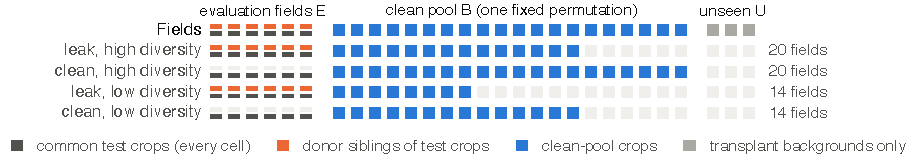
\includegraphics[width=\linewidth]{figures/design.pdf}
\caption{The 2C factorial for one seed. Every cell shares the same test crops (half of each
evaluation field's crops). Leak cells add the evaluation fields' remaining sibling crops;
clean cells use other fields instead. Within a diversity level, crop and field counts are
identical; low-diversity field sets are nested inside high-diversity ones.}
\label{fig:design}
\end{figure}

The 2C factorial (Figure~\ref{fig:design}) fixes one test set per seed and varies only the
training set. Thirty percent of SIPaKMeD fields with at least two crops are evaluation
fields; half of each one's crops (rounded down) form the common test set (about 527
crops) and the rest are its \emph{donor siblings}. Six fields per class are reserved as
unseen background donors for Section~\ref{sec:transplant}. Four training sets each hold
exactly 220 crops per class. The clean cells draw only from non-evaluation fields; the
leak cells replace the last $|E|$ fields of the same random permutation with the
evaluation fields' donor siblings. High-diversity cells use 720 distinct fields and
low-diversity cells 504, a 1.43-fold contrast that brackets the natural 1.18. Within a
diversity level, leak and clean therefore have the same crop count, the same number of
distinct fields, and the same allocation rule; they differ only in whether the test
fields' siblings are present. ResNet-50, DenseNet-121, ConvNeXt-T, and ViT-B/16 are
trained on all four cells for ten seeds (160 runs). H3 is the leak main effect in
\begin{equation}
\text{acc} \sim \text{leak}\times\text{div} + (1+\text{leak}\mid\text{architecture}) + (1\mid\text{seed}) + (1\mid\text{training set}).
\end{equation}
Because the low-diversity leak cell gives each test crop more training siblings (3.0
versus 2.0), the diversity effect is estimated within clean cells only and the interaction
is exploratory.

\subsection{Counterfactual background transplants (H4)}
\label{sec:transplant}

Every 2C model is also evaluated on composites of its test set. Each test cell's
foreground (the Study~1 background-only mask) is feathered onto the inpainted background
of a donor crop: its own background (\emph{self}, which isolates seam and inpainting
artifacts), a sibling from the same field (\emph{sibling}), an unseen field of the same
class (\emph{unseen same-class}), and unseen fields of every other class. Leak models have
seen each test cell's field context with the correct label; clean models have not. The
per-run quantity $\text{route} = \text{acc(sibling)} - \text{acc(unseen same-class)}$
measures how much the cell's own acquisition context contributes beyond class-typical
context, and H4 is its leak-minus-clean difference:
\begin{equation}
\text{route} \sim \text{leak} + \text{div} + (1+\text{leak}\mid\text{architecture}) + (1\mid\text{seed}) + (1\mid\text{training set}).
\end{equation}
The ratio of H4 to the leakage effect on unmodified images estimates the share of the
inflation carried by the context route. The probability shift toward the donor class
under other-class backgrounds measures, separately, whether classifiers read class
information from backgrounds at all.

\subsection{Adversarial fingerprint suppression (H5)}
\label{sec:grl}

A two-layer parent-identity head is attached to the penultimate features through a
gradient-reversal layer~\citep{ganin2015backprop,ganin2016dann}, with the DANN ramp
reaching a maximum coefficient $\lambda\in\{0,0.01,0.03,0.1,0.3,1,3\}$. The head only
discriminates fields \emph{within} the sample's class, so suppressing it never requires
removing class information. ResNet-50 and ConvNeXt-T are trained on the natural P1 and P2
splits of ten seeds (280 runs). Fingerprint recoverability $R$ is the within-class
field-identification accuracy of a logistic-regression probe on frozen features of the
balanced 424-field probe crops, reported against its class-only floor. Within the
non-degenerate regime (mean P2 accuracy within 1~pp of $\lambda=0$), and provided
suppression removes at least a quarter of the above-floor recoverability, H5 is a positive
slope of the per-seed P1--P2 gap on $R$. If the shortcut account is right, the gap closes
as the fingerprint is suppressed while P2 accuracy stays flat; if P1 stays inflated while
$R$ collapses, the gap is something else.

\subsection{CRIC (H2)}
\label{sec:cric}

CRIC cells are $100\times100$ windows centred on the published nucleus coordinates of
the 400 Figshare slide images (six Bethesda classes). ResNet-18, ResNet-50, DenseNet-121,
EfficientNet-B0, ConvNeXt-T, and ViT-B/16 are trained on P1, P1-prime (which differs from P1
by 2--11 training cells), and P2 for ten seeds (180 runs). H2 applies~\eqref{eq:h1} to CRIC
accuracy.

\subsection{Multiplicity}

H1 is the single primary endpoint. H2--H5 form one Holm family~\citep{holm1979}
(family-wise $\alpha=0.05$); each is supported only if its adjusted $p<0.05$ and its estimate
has the predicted sign. All other analyses are secondary or exploratory.

\section{Results}
\label{sec:results}
[Pending: registered Study 2 results.]


\bibliographystyle{unsrtnat}
\bibliography{references}

\appendix
\section{Post hoc omnibus reanalysis of Study 1}
\label{app:pilot}
Fitting model~\eqref{eq:h1} to the 60 Study~1 P1 and P2 runs (six architectures, five seeds)
gives a P1--P2 difference of \PilotEst~pp (SE \PilotSE, Satterthwaite $p=\PilotP$,
$\mathrm{df}=\PilotDf$). This analysis was specified after the Study~1 data were seen; it
motivated Study~2 and supplied its pilot variance components, and it is not confirmatory.

\section{Power analysis}
\label{app:power}
\begin{figure}[h]
\centering
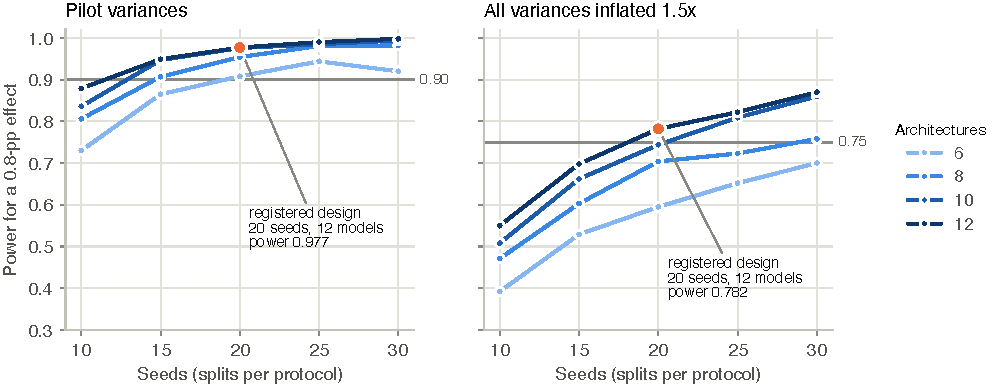
\includegraphics[width=\linewidth]{figures/power.pdf}
\caption{Simulated power of model~\eqref{eq:h1} for a 0.8-pp effect (1,000 simulations per design).
The registered design (twenty seeds, twelve architectures) reaches \PowerChosen{} with pilot
variances and \PowerInflated{} with every variance inflated by half.}
\label{fig:power}
\end{figure}


\end{document}
